
\documentclass{scrreprt}
\usepackage{scrhack} 

%%% PACKAGES %%%%%%%%%%%%%%%%%%%%%%%%%%%%%%%%%%%%%%%%%%%%%%%%%%%%%%%%%%
% inputenc allows the usage of non-ascii characters in the LaTeX source code
\usepackage[utf8]{inputenc}
% Language
\usepackage[ngerman]{babel}
% Import graphics
\usepackage{graphicx}
% Links
\usepackage{xurl}
\usepackage{hyperref}
% Zeilenabstand
\usepackage{setspace}
% Textfarbe
\usepackage{xcolor}

% Code Beispiele
\usepackage{listings}
\definecolor{keywords}{RGB}{255,0,90}
\definecolor{comments}{RGB}{0,0,113}
\definecolor{red}{RGB}{160,0,0}
\definecolor{green}{RGB}{0,150,0}
\lstset{language=Python, 
        basicstyle=\ttfamily\small, 
        keywordstyle=\color{keywords},
        commentstyle=\color{comments},
        stringstyle=\color{red},
        showstringspaces=false,
        identifierstyle=\color{green},
        }

% damit Latex nicht die Kapitel 1, 2, ... als 0.1, 0.2, ... schreibt
\renewcommand{\thesection}{\arabic{section}}

\usepackage{fancyvrb}
\renewcommand{\FancyVerbFormatLine}[1]{%
  \ifnum\value{FancyVerbLine}<5\color{red}#1%
  \else\color{blue}#1\fi}

%%% TITLEPAGE %%%%%%%%%%%%%%%%%%%%%%%%%%%%%%%%%%%%%%%%%%%%%%%%%%%%%%%%%%%%%%%%%
\subject{Berichts-Handout}
% head line of the title page, here with department and logo
\titlehead{%
  \begin{minipage}{.7\textwidth}%
  Humboldt-Universit\"at zu Berlin\\
  Mathematisch-Naturwissenschaftliche Fakult\"at\\
  Institut f\"ur Mathematik
  \end{minipage}
  \begin{minipage}{.29\textwidth}%
    \begin{flushright}
      \includegraphics*[scale=.6]{husiegel_bw.pdf}%
    \end{flushright}
  \end{minipage}
}
% title of the document
\title{Untersuchung der harmonischen Reihe}
%  subtitle
\subtitle{Arbeitsblatt 3}
% authors
\author{%
  Chantal Gerth, Alina Apel\\635838, 614787\\ \\Gruppe 22
}
% date of submission
\date{}


%%% BEGIN OF DOCUMENT %%%%%%%%%%%%%%%%%%%%%%%%%%%%%%%%%%%%%%%%%%%%%%%%%%%%%%%%%
\setstretch{1.25}
% the type-setting of the document starts here
\begin{document}
% generating the title page
\maketitle
% generating the table of contents (requires to run pdflatex twice!)
\tableofcontents
\thispagestyle{empty}



%%% BEGIN OF CONTENT %%%%%%%%%%%%%%%%%%%%%%%%%%%%%%%%%%%%%%%%%%%%%%%%%%%%%%%%%%
\newpage

\section{Einführung und Motivation}
Im heutigen Zeitalter werden Computer in fast allen Lebensbereichen genutzt. Daher ist es besonders wichtig, dass der Computer korrekt rechnet. Leider tut er das nicht immer. Ein anschauliches Beispiel dafür ist die harmonische Reihe. Deswegen geht es in diesem Experiment darum, die Konvergenz der harmonischen Reihe mit verschiedenen Algorithmen und Datentypen zu untersuchen und dies mit dem analytischen Ergebnis zu vergleichen.

\section{Theoretische Grundlagen} \label{sec:theorie}
Die harmonische Reihe ist eine unendliche Reihe der Form
\[
\sum_{n=1}^{\infty} \frac{1}{n},
\]
die aus den Kehrwerten natürlicher Zahlen besteht. Mathematisch gesehen divergiert die harmonische Reihe, was bedeutet, dass die Summe der Reihe gegen Unendlich strebt, wenn die Anzahl der Terme zunimmt. Beim Berechnen der Partialsummen der harmonischen Reihe durch einen Computer kann es allerdings zu Rundungsfehlern kommen, die durch die begrenzte Genauigkeit der Fließkommazahlen verursacht werden. Je nach Datentyp wird n so groß und damit der auf die vorherige Partialsumme aufzuaddierende Summand so klein, dass die Bitmuster der entsprechenden Datentypen nicht mehr ausreichen, um diese numerisch kleine Zahl darzustellen. Der entsprechende Summand wird deshalb auf 0 gerundet. Für höhere n wird dann nur noch 0 aufaddiert, sodass die Folge der Partialsummen zu konvergieren scheint. Die Genauigkeit der Ergebnisse hängt dabei vom verwendeten Datentyp und Algorithmus ab. Je weniger Nachkommastellen das Bitmuster eines Datentyps darstellen kann, desto früher tritt das Problem auf. Schlussendlich trat in allen von uns untersuchten Beispielen diese Konvergenz auf, obwohl die Reihe selbst divergiert.

\section{Experiment} \label{sec:experiment}
\begin{figure}
    \centering
    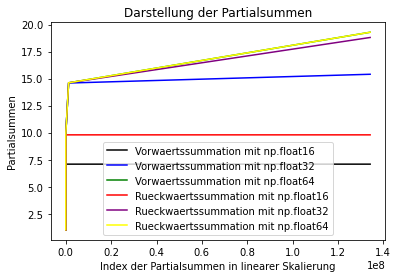
\includegraphics[width=0.9\textwidth]{plot_basis8_endwert9.png}
    \caption{Basis 8, Startwert 0, Endwert 9, Num 5}
    \label{fig:basis8}
    \vspace*{15mm}
    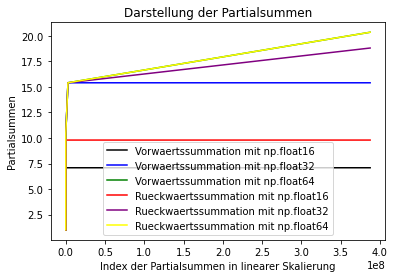
\includegraphics[width=0.9\textwidth]{plot_basis9_endwert9.png}
    \caption{Basis 9, Startwert 0, Endwert 9, Num 5}
    \label{fig:basis9}
\end{figure}

Unser Programm \texttt{main.py} ist ein Experimentierskript für den Nutzer. Es gibt die Möglich-keit, eine gewisse Anzahl an Partialsummen zu berechnen, grafisch darzustellen und zu speichern/abzurufen. Dabei kann der Nutzer Standardparameter wählen oder eigene Parameter eingeben. \\

\noindent Für die Berechnung wird ein Anfangswert und ein Endwert, sowie eine Basis benötigt. Dann kann der Nutzer wählen, wie viele Partialsummen er berechnet haben will. Die Eingabe der Parameter erfolgt über den Terminal. Dafür wird die Funktion read\textunderscore number aus dem Modul tools\textunderscore read\textunderscore save (\autoref{sec:toolsreadsave}) genutzt. Wählt der Nutzer die vordefinierten Parameter, wird mit \texttt{start = 1, stop = 5, basis = 10, num = 10} fortgefahren. \\

\noindent Anschließend berechnet das Programm durch Vorwärtssummation und Rückwärtssummation mit den Datentypen \texttt{np.float16}, \texttt{np.float32} und \texttt{np.float64} die Partialsummen und stellt die Ergebnisse graphisch dar. Hat der Nutzer angegeben, dass die berechneten Partialsummen gespeichert werden sollen, werden die Ergebnisse mit der Funktion  save\textunderscore data aus dem Modul tools\textunderscore read\textunderscore save (\autoref{sec:toolsreadsave}) in eine CSV-Datei exportiert. \\

\noindent Entsprechend dieses Arbeitsablaufs wurden für die Untersuchung der Konvergenz der harmonischen Reihe folgende Berechnungen durchgeführt: 

\begin{itemize}
    \item Basis 8, Startwert 0, Endwert 9, 5 Partialsummen
    \item Basis 9, Startwert 0, Endwert 9, 5 Partialsummen
\end{itemize}

\noindent Die Ergebnisse sind in \autoref{fig:basis8} und \autoref{fig:basis9} graphisch dargestellt. Eine Wahl höherer Parameter war aufgrund der Laufzeit des Programms nicht möglich. In den Grafiken ist dennoch das theoretisch zu erwartende Problem, welches in \autoref{sec:theorie} beschrieben wurde, ersichtlich: Die Reihe scheint für die Datentypen \texttt{np.float16}, \texttt{np.float32} zu konvergieren.

\section{Schlussfolgerung}
Basierend auf den Ergebnissen unseres Experiments lässt sich feststellen, dass die harmonische Reihe aufgrund von Rundungsfehlern und begrenzter Genauigkeit der Fließkommazahlen auf Computern scheinbar konvergiert, obwohl sie theoretisch divergiert. Insbesondere zeigt sich, dass die Genauigkeit der Berechnung von der Wahl des Datentyps und des verwendeten Algorithmus abhängt. Während die Vorwärtssummation mit dem Datentyp \texttt{np.float32} die geringste Genauigkeit aufweist, liefert die Rückwärtssummation mit dem Datentyp \texttt{np.float64} das genaueste Ergebnis. Diese Erkenntnisse regen dazu an, weitere Optimierungen zu untersuchen, um möglicherweise eine Divergenz der harmonischen Reihe auf dem Computer nachzuweisen.

\newpage

\section{Python-Dokumentation tools\textunderscore read\textunderscore save} \label{sec:toolsreadsave}
Das Modul \texttt{tools\textunderscore read\textunderscore save.py} dient der Modularisierung häufig verwendeter Funktionen zur Nutzerinteraktion. Das Programm implementiert drei Funktionen: \texttt{read\textunderscore number} zum Einlesen von Nutzereingaben, \texttt{save\textunderscore data} zum Abspeichern von Listen in .csv-Dateien, und \texttt{load\textunderscore data} zum Einlesen von Daten aus .csv-Dateien. \\

\subsection{Schnittstellendokumentation}
\subsubsection{read\textunderscore number}
Liest eine Zahl vom Benutzer ein, die innerhalb der angegebenen Grenzen liegt und in den gewünschten Datentyp konvertiert werden kann. \\

\noindent \textbf{Parameter:}
\begin{itemize}
    \item \texttt{question} (str): Eingabeaufforderung an den Benutzer.
    \item \texttt{data\textunderscore type} (type): Gewünschter Datentyp der Eingabe.
    \item \texttt{lower\textunderscore limit} (float): Untere Grenze der gültigen Eingabe (Standardwert: -$\infty$).
    \item \texttt{upper\textunderscore limit} (float): Obere Grenze der gültigen Eingabe (Standardwert: $\infty$).
\end{itemize}

\noindent \textbf{Rückgabewert:}
\begin{itemize}
    \item Die eingegebene Zahl im gewünschten Datentyp.
\end{itemize}

\noindent \textbf{Ausnahmen:}
\begin{itemize}
    \item \texttt{ValueError}: Wenn eine leere Eingabe gemacht wird.
\end{itemize}

\noindent \textbf{Beispiel:} \\
Nachfolgend wird die verwendung der Funktion im Experimentierskript zur Konvergenz der harmonischen Reihe (\autoref{sec:theorie}) gezeigt:
\begin{lstlisting}
num = read_number(question = "Anzahl der zu berechnenden Partialsummen: ", 
                  data_type = int, 
                  lower_limit = 2)
\end{lstlisting}

\noindent \textbf{Programmablauf:} \\
Im nachfolgenden Fließdiagramm ist dargestellt, wie die Funktion sicherstellt, dass die Eingabe des Nutzers den gewünschten Anforderrungen entspricht, bevor der eingelesene Wert zurückgegeben wird.

\begin{figure}
    \centering
    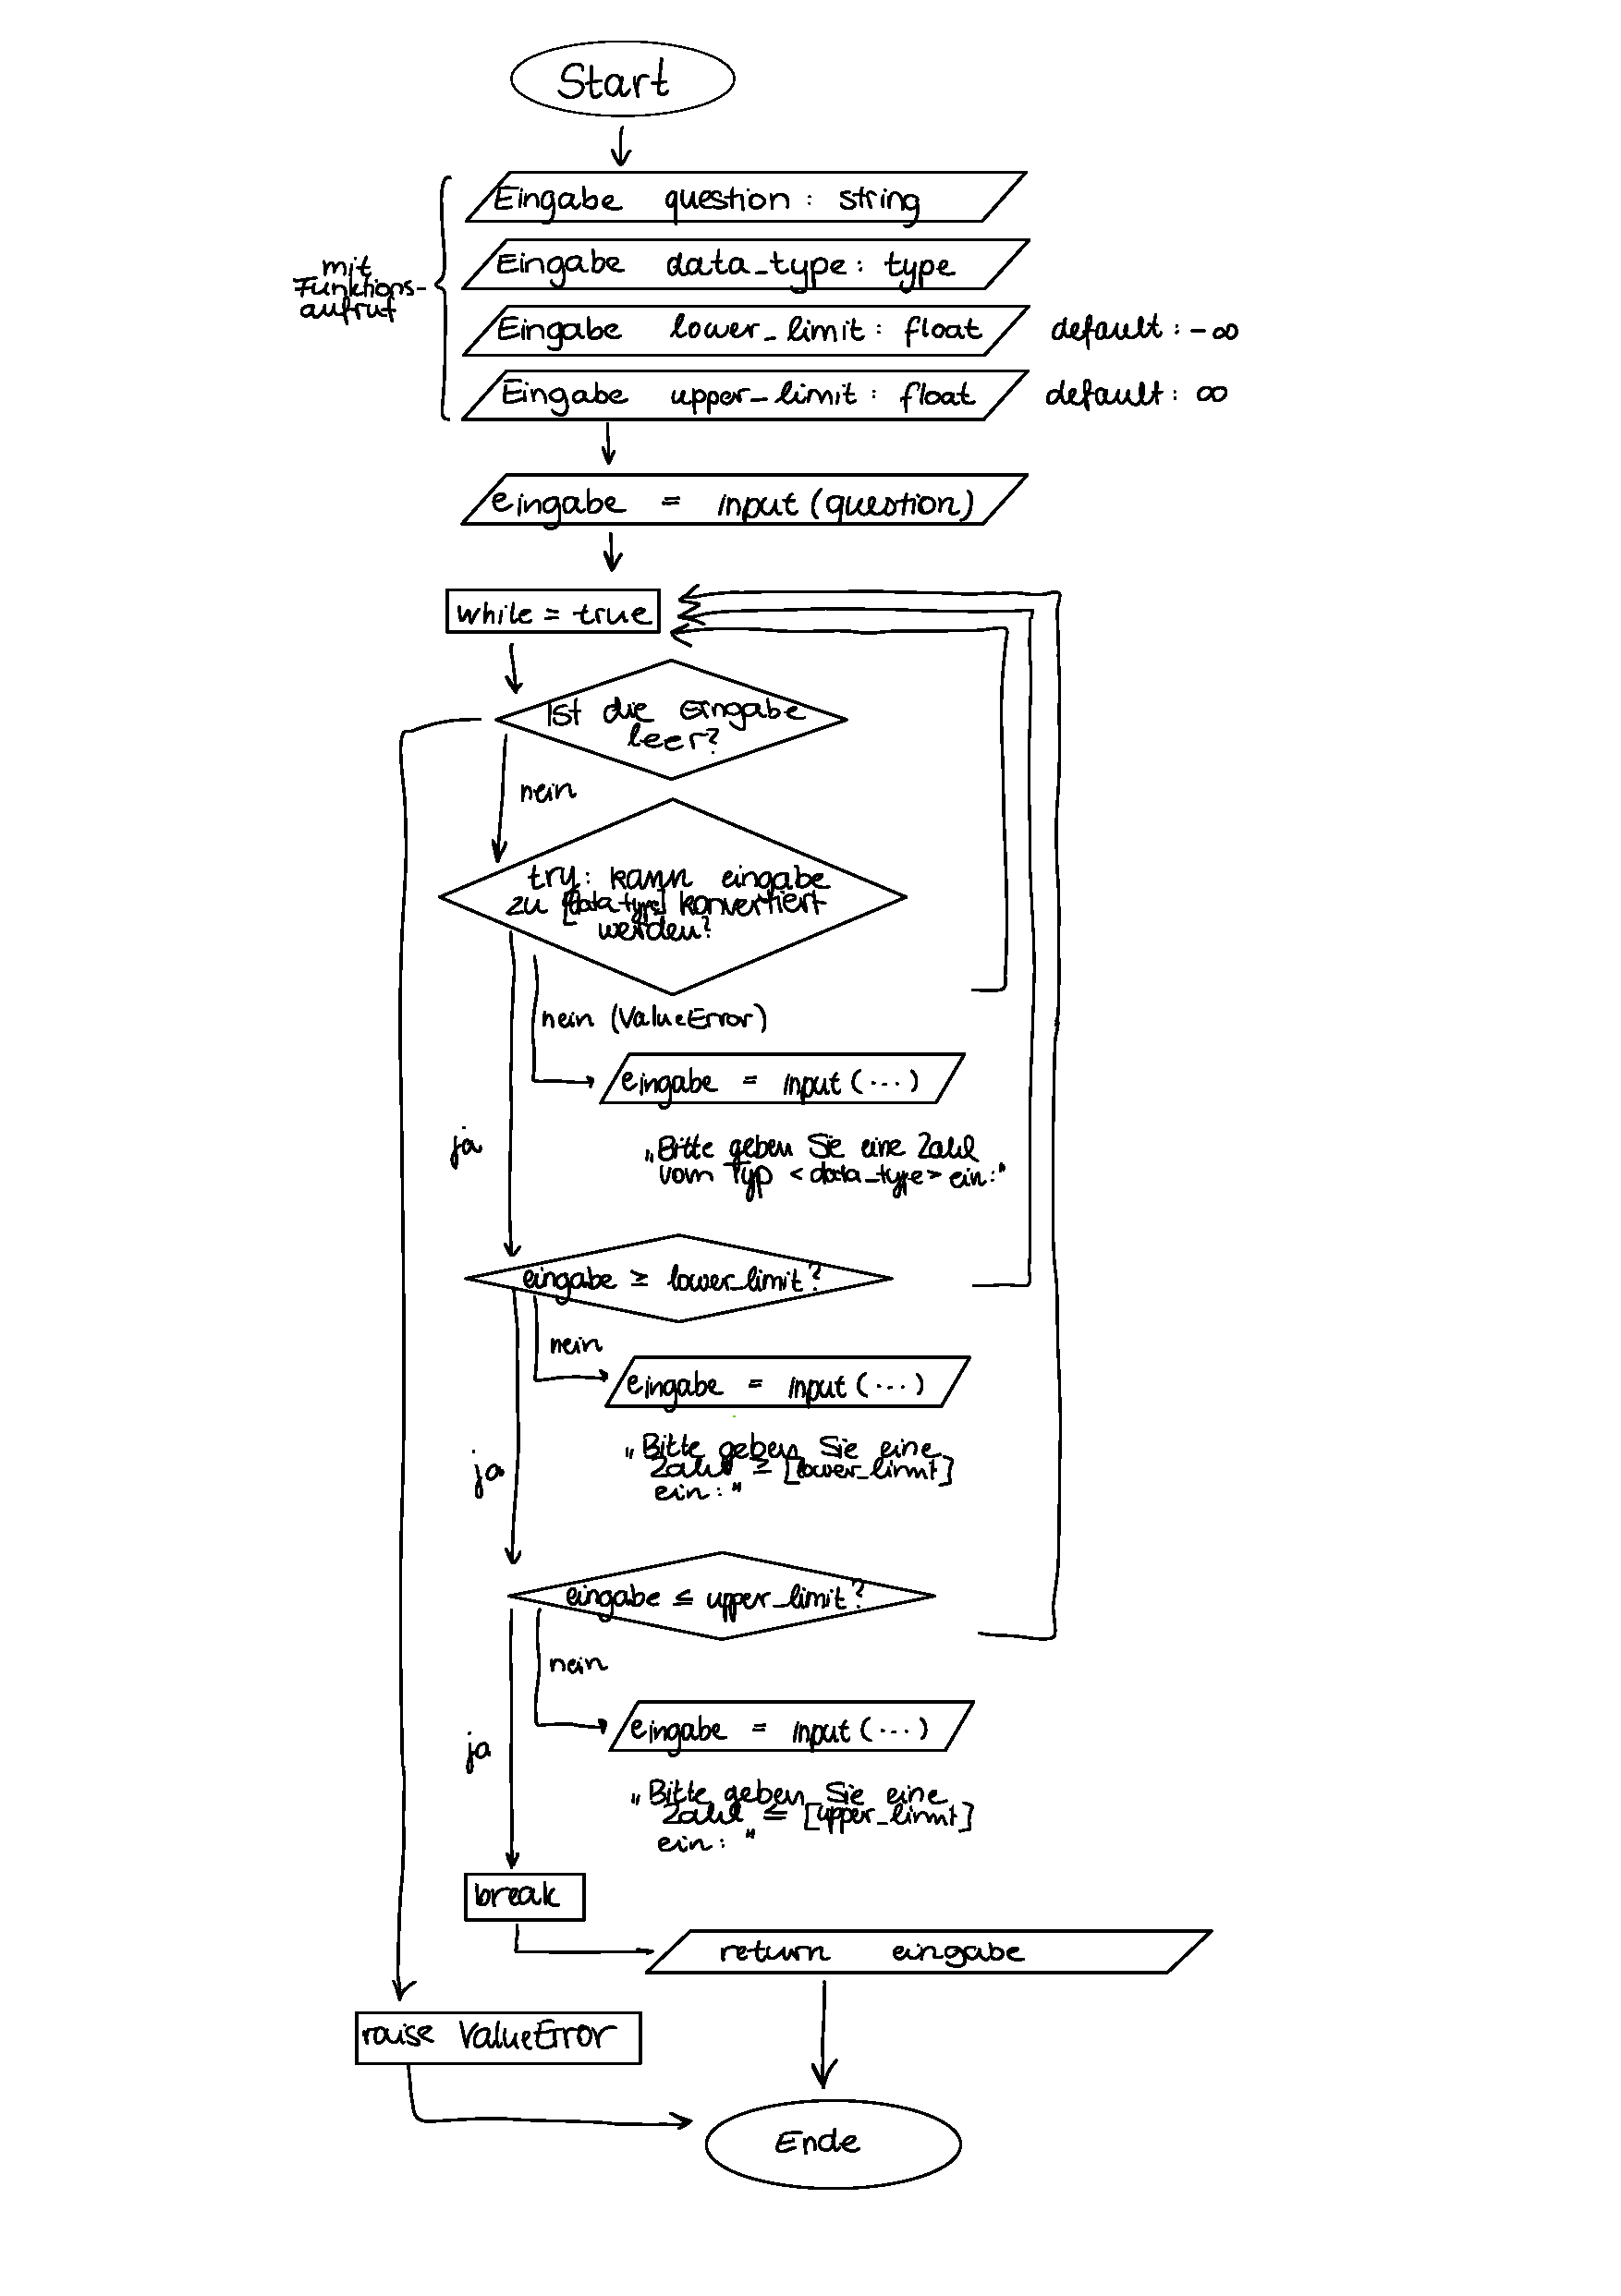
\includegraphics[width=0.8\textwidth]{AB3-flow_cropped.pdf}
    \caption{Fließdiagramm zum Ablauf von read\textunderscore number}
\end{figure}


\subsubsection{save\textunderscore data}
Speichert eine Liste von Zahlen in eine CSV-Datei mit \texttt{","} als Trennzeichen. \\

\noindent \textbf{Parameter:}
\begin{itemize}
    \item \texttt{data}: Eine Liste von Zahlen.
    \item \texttt{filepath} (str): Pfad der zu speichernden Datei.
\end{itemize}

\noindent \textbf{Ausnahmen:}
\begin{itemize}
    \item \texttt{RuntimeError}: Wenn das Speichern fehlschlägt.
\end{itemize}

\noindent \textbf{Beispiel:} \\
Nachfolgend wird die verwendung der Funktion im Experimentierskript zur Konvergenz der harmonischen Reihe (\autoref{sec:theorie}) gezeigt:
\begin{lstlisting}
save_data(result_vorwaerts_float16,
          "convergence_data_export/result_vorwaerts_float16.csv")
\end{lstlisting}

\vspace{10mm}

\subsubsection{read\textunderscore data}
Liest eine Liste von Zahlen aus einer CSV-Datei mit \texttt{","} als Trennzeichen ein. \\

\noindent \textbf{Parameter:}
\begin{itemize}
    \item \texttt{filepath} (str): Pfad der zu lesenden Datei.
\end{itemize}

\noindent \textbf{Rückgabewert:}
\begin{itemize}
    \item Eine Liste von Zahlen.
\end{itemize}

\noindent \textbf{Ausnahmen:}
\begin{itemize}
    \item \texttt{RuntimeError}: Wenn das Einlesen fehlschlägt.
\end{itemize}

\noindent \textbf{Beispiel:} \\
Nachfolgend wird die verwendung der Funktion im Experimentierskript zur Konvergenz der harmonischen Reihe (\autoref{sec:theorie}) gezeigt:
\begin{lstlisting}
result_vorwaerts_float16 = load_data("convergence_data_import/
                                      result_vorwaerts_float16.csv")
\end{lstlisting}

\subsection{Nutzungshinweise und Hauptprogramm}
In tools\textunderscore read\textunderscore save.py ist eine main() Funktion implementiert. Sie dient der Demonstration der
enthaltenen Funktionen und wird nur ausgeführt, wenn tools\textunderscore read\textunderscore save.py direkt mittels python3 tools\textunderscore read\textunderscore save.py gestartet wird. \\

\noindent Dabei wird der Nutzer zuerst aufgefordert, eine ganze Zahl zwischen 3 und 7 in den Terminal einzugeben, um read\textunderscore number zu testen. Eine leere Eingabe beendet das gesamte Testprogramm.

\begin{lstlisting}
def main():
    """Anwednungsbeispiele"""
    # read_number()
    print("Zunächst wird die Funktion load_data() getestet.")
    print("Eine leere Eingabe ermöglicht den Abbruch und führt 
           zum Test der nächsten Funktion.")

    anfrage = "Bitte geben Sie eine ganze Zahl x mit 3 <= x <= 7 ein."
    
    try: 
        eingabe_zahl = read_number(anfrage, int, lower_limit=2)
        print("")
        print("Die Funktion gibt zurück: " 
               + str(eingabe_zahl) 
               + ", Datentyp: " 
               + str(type(eingabe_zahl)))
    except ValueError:
        print("Abbruch des Tests.")
        exit()
\end{lstlisting}

\noindent Anschließend wird save\textunderscore data durch Speichern einer vordefinierten Liste demonstriert: 

\begin{lstlisting}

    # save_data()
    print("")
    print("Nun wird eine Beispielliste erstellt und exportiert:
           [1.1117634, 2.55, 3.3, 144.0]")
    liste = [1.1117634, 2.55, 3.3, 144.0]
    try:
        save_data(liste, "test.csv")
    except RuntimeError:
        print("Speichern der Liste fehlgeschlagen.")
\end{lstlisting}

\noindent Zuletzt wird read\textunderscore data demonstriert, indem die zuvor gespeicherte Liste wieder eingelesen wird:

\begin{lstlisting}
    # load_data()
    print("")
    print("Dieselbe Liste wird nun wieder eingelesen und ausgegeben.")
    try:
        print(load_data("test.csv"))
    except RuntimeError:
        print("Einlesen der Datei fehlgeschlagen.")
\end{lstlisting}


\begin{thebibliography}{99}

\bibitem{pakin} NumPy Developers, \emph{NumPy documentation} (2022). \url{https://numpy.org/doc/1.26/}

\bibitem{wikipedia1} \emph{Harmonische Reihe.} Wikipedia [online] \url{https://de.wikipedia.org/wiki/Harmonische_Reihe}

\bibitem{pakin} Scott Pakin, \emph{The Comprehensive \LaTeX{} Symbol List} (2024). \url{https://tug.ctan.org/info/symbols/comprehensive/symbols-a4.pdf}

\bibitem{pakin} Hella Rabus, \emph{Einführung in das Wissenschaftliche Rechnen, Skript zur Vorlesung} (2024). \url{https://moodle.hu-berlin.de/mod/folder/view.php?id=4331460}

\end{thebibliography}

\newpage

\noindent \textbf{Selbstständigkeitserklärung}
\\ \\
Ich versichere, dass ich in dieser schriftlichen Studienarbeit alle von anderen Autor:innen wörtlich übernommenen Stellen wie auch die sich an die Gedankengänge anderer Autoren:innen eng anlehnenden Ausführungen meiner Arbeit besonders gekennzeichnet und die entsprechenden Quellen angegeben habe. Zusätzlich führe ich den Einsatz von IT-/KI-gestützten Schreibwerkzeugen zur Anfertigung dieser Arbeit im Abschnitt „Übersicht verwendeter Hilfsmittel“ im Anhang des eingereichten pdf-Dokumentes vollständig auf. Hierin habe ich die Verwendung solcher Tools vollständig durch Angabe ihres Produktnamens, meiner Bezugsquelle (z.B. URL) und Angaben zu genutzten Funktionen der Software sowie zum Nutzungsumfang dokumentiert. Bei der Erstellung dieser Studienarbeit habe ich durchgehend eigenständig und beim Einsatz IT-/KI-gestützter Schreibwerkzeuge steuernd gearbeitet. \\ \\ \\ \\


\noindent Chantal Gerth, Berlin, 21.05.2024 \\ \\ \\ \\

\noindent Alina Apel, Berlin, 21.05.2024 \\

%%% END OF DOCUMENT %%%%%%%%%%%%%%%%%%%%%%%%%%%%%%%%%%%%%%%%%%%%%%%%%%%%%%%%%%%
\end{document}

